\clearpage
\section{散点数据的处理和方法介绍}
\subsection{散点数据的处理}
\par 数据作为多种维度的信息,在数据表现上主要依靠图表展示。而散点图的数据分析方法主要是基于数值层面的方法、基于形状模式的方法、基于人对散点图的感知情况的方法。在数据展示的可视化处理上,比如散点图矩阵,就是将二维散点图进行重复排列,用户很容易理解。但当维数增多时,大量的散点图需要一定的展示空间,而且其数据分布也不容易被用户观察到。因此,许多工作着眼于识别大量散点图中用户感兴趣的散点图子集,并将子集呈现给用户。
\begin{table}[!ht]
    \centering
        \caption{各地域的经纬度地址}
    \begin{tabular}{ccccccccc}
    \hline
       区县  &  杭州市 &	上城区	& 下城区 &	江干区 & 拱墅区 & 西湖区	& 滨江区	& 萧山区\\ \hline
       经度  &  120.15 &	120.17	& 120.17 &	120.2 & 120.13 & 120.13	& 120.2	& 120.27 \\ 
       纬度  & 30.28  &	30.25	& 30.28 &	30.27 & 30.32 & 30.27	& 30.2	& 30.17 \\ \hline
    \end{tabular}
    \label{tab:my_label}
\end{table}

\begin{table}[!ht]
    \centering
     \caption{各地域的经纬度地址}
    \begin{tabular}{ccccccccc}
    \hline
       区县  &  余杭区 &	...	& 桐庐县 &	淳安县 & 建德市 & 富阳市	& 临安市	& 宁波市\\ \hline
       经度  &  120.3 &	...	& 119.67 &	119.03 & 119.28 & 119.95	& 119.72	& 121.55 \\ 
       纬度  & 30.42  &	...	& 29.8 &	29.67 & 29.48 & 30.05	& 30.23	& 29.88 \\ \hline
    \end{tabular}
    \label{tab:my_label}
\end{table}

\par 在地域的分类划分聚类中,就采用先呈现子集并聚类后分析的方法。如图2-1浙江省县市中心的地域分布图。

\begin{figure}[!ht]
    \centering
     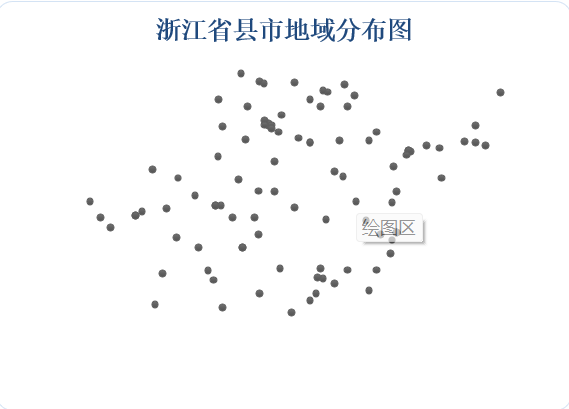
\includegraphics[width=0.5\textwidth]{fig2/fig21.png}
      \caption{浙江省县市中心的地域分布图}
\end{figure}
\FloatBarrier  %禁止图片浮动

\subsection{\rm{K-Means}聚类算法}
\subsubsection{算法简介}
\par K-Means算法(也叫$k$均值或$k$平均算法),是机器学习领域常见的一种无监督学习模型,其将距离作为相似性评价指标。在K-Means算法中,将距离较近的同类数据点放入一个簇内,且它们之间的距离应尽可能地接近;而不同簇的中心距离则应尽可能地远。
K-Means是一种广泛应用于配送网络末端配送区域划分的聚类算法。本文使用的算法根据预设的$m$个聚类中心对样本点进行聚类划分后,根据得到的每个类中点的平均值重新作为下次聚类划分的聚类中心,不断重复聚类划分的过程直到聚类中心不再发生变化,算法终止输出最优聚类结果。算法的目标是使聚类结果各类中的点尽可能的紧凑,并且使不同类别之间相互分开。

\subsubsection{算法过程}
\par 对数据进行基本处理后,计算其中各点的均值:

\begin{equation}
    \overline{x_i} = \frac{1}{n}\sum_{i=1}^na_{ij}
\end{equation}
\par 计算各个数据的具体的相对中心点的的位置:
 \begin{equation}
    z_i=\sqrt{\frac{1}{n-1}\sum_{i=1}^n(a_{ij}-\overline{x_i})^2}
\end{equation}
\par 计算出各个样本点两两之间的距离,并构造距离矩阵$(_{ik})_{n \times n}$ 。采用欧几里得距离:
 
\begin{equation}
    d_{ik} = \sqrt{\sum_{j=1}^m(z_{ij}-z_{kj})^2}
\end{equation}
\par 构造$n$个类且每个类只包含一个样本点,每一个类的平台高度为零。再合并距离最近的两类为新类,且这两类之间的距离值作为聚类图中的平台高度。最后,绘制出聚类图,选择所需要的决定类的个数和类。由于算法在聚类时需要先进行聚类中心的初始化,所以会导致聚类的不稳定;又因为每次迭代前都需要重新计算聚类中心,也增加了算法的时间复杂度。针对以上问题,所以采用模糊聚类的算法进行改进。

\subsection{模糊K-Means聚类算法}
\par 在K-Means算法下,每一个数据点$x$在分类时,均会被严格地放入某一个类别中。但在实际的分类过程中,这一个数据点$x$却难以严格地被划分到同一个类别中,其可能是以不同的隶属度划分到某一类。此时,对每一个分类结果均可用一个模糊分类矩阵表示:

\begin{equation}
U=\begin{bmatrix}
u_{11} & u_{12} & \cdots & u_{1n}\\
u_{21} & u_{22} & \cdots & u_{2n} \\
\vdots  & \vdots  & \ddots  &\vdots  \\
u_{c1} & u_{c2} & \cdots & u_{cn} \\
\end{bmatrix}
\end{equation}

\par 其中,$u_{ij} \in [0,1]$ 表示某个数据点对于该类别的隶属度。定义模糊分类下的误差平方准则函数为:
\begin{equation}
I_{m}=\sum_{i=1}^{c} \sum_{j=1}^{n} u_{i j}^{i m}\left\|\left|x_{j}-w_{i} \|\right|^{2}\right.
\end{equation}

\par 在计算聚类中心时,也需要进行模糊化处理:
\begin{equation}
    w_{i}(t)=\frac{\sum_{j=1}^{n}u_{ij}^{m}x_{j}}{\sum_{j=1}^{n}u_{ij}}
\end{equation}
在迭代过程中,需要对模糊矩阵进行修正,直至最后得出结果:
 
\begin{equation}
    u_{ij}(t+1) = \frac{1}{\sum_{i=1}^{c} (\left \| \left | \frac{x_{j}-w_{j}  }{x_{j}-w_{i}}  \right |  \right \| )^{\frac{z}{m-i}}} 
    \end{equation}
\subsection{散点分布的可视化}
\par 为了协助人们对数据的分析,将分析结果可视化是重要的。在清晰表达信息给读者时,在二维图像上能够提供更直观的信息表现。由于信息的数据反映在很大程度上取决于了表达方式,所以在分析由数字和列表组成的数据时。数据可视化的本质是展现数据,数据可视化是以图形的方式清晰有效地传达和传播信息。赋予了可视化数据的价值,帮助读者更好的从信息中提取,从图像中收获价值。
其中JavaScript语言可以对收集到的数据中的经纬度进行坐标映射转换为地图中的对应坐标值。再通过自建函数调用参数处理传入的参数数据,进而绘制出最后的结果。

\subsection{TSP算法}
\par 意大利学者\rm{Dorigo}等人提出了第一个蚁群算法—蚂蚁系统,并用于\rm{TSP}问题的求解。由于每只蚂蚁都可通过一种称为信息素的媒介来交流信息,指导自己选择下一步所要行走的路径。蚂蚁在行走过程中会在路径上释放信息素,因此每条路径都会被信息素所标记,蚂蚁可以检测信息素浓度,并以一定的概率朝着信息素浓度高的地方移动。这是一种正反馈机制,越多的蚂蚁选择相同的路径,则这条路径被选择的概率就越高,吸引更多的蚂蚁选择相同的路径,最终蚂蚁往返于巢穴到食物源间的最短路径。
\par 经过大量学者进行不断的优化,使\rm{Shelokar}将蚁群算法成功应用于求解聚类问题,从此开始了蚁群算法在聚类问题的应用。蚁群算法具有分布计算、信息正反馈和启发式搜索的特征,本质上是进化算法中的一种启发式全局优化算法。但是其在解决大型优化问题时,存在搜索空间和时间性能上的矛盾,易出现过早收敛于非全局最优解以及计算时间过长的弱点。近年来,依据蚁群算法求解问题的基本模型和流程,为能够加快蚁群算法收敛速度、提高算法的运行性能、避免局部最优和提高全局搜索能力等,主要的改进策略主要有三方面:蚁群算法的信息素更新策略改进、路径的选择策略改进、蚁群算法与其他算法的融合。由于蚁群算法模型会随着问题变化而略有改动,因此这一部分以求解TSP问题为线索介绍蚂蚁系统。